\section{HLS and VideoJS}
\label{sec:HLS and VideoJS}

https://github.com/videojs/video.js
https://github.com/videojs/videojs-contrib-hls

HTTP Live Streaming (HLS) has become a de-facto standard for streaming video on mobile devices. In order to use this standard in X-Learning platform i exploit the Video.js that is s a free and open source library.
Video.js is a web video player built from the ground up for an HTML5 world. It supports HTML5 and Flash video, as well as YouTube and Vimeo (through plugins). It supports video playback on desktops and mobile devices. This project was started mid 2010, and the player is now used on over 200,000 websites.
HTTP Live Streaming (HLS) has standard for streaming video thanks to its native support on iOS and Android. There are a number of reasons independent of platform to recommend the format, though:
Supports (client-driven) adaptive bitrate selection
Delivered over standard HTTP ports
Simple, text-based manifest format
No proprietary streaming servers required
Unfortunately, all the major desktop browsers except for Safari are missing HLS support. That leaves web developers in the unfortunate position of having to maintain alternate renditions of the same video and potentially having to forego HTML-based video entirely to provide the best desktop viewing experience.
This tech attempts to address that situation by providing a polyfill for HLS on browsers that have Flash support. You can deploy a single HLS stream, code against the regular HTML5 video APIs, and create a fast, high-quality video experience across all the big web device categories.
The videojs-hls tech use in my project  is still working towards a 1.0 release so it may not fit your requirements today. Specifically, there is no support for:
Alternate audio and video tracks
Subtitles
Segment codecs other than H.264 with AAC audio
Internet Explorer < 10

\subsection{Adaptive Switching Behavior}
\label{sec:Adaptive Switching Behavior}

https://github.com/videojs/videojs-contrib-hls/blob/master/docs/bitrate-switching.md


The HLS tech tries to ensure the highest-quality viewing experience possible, given the available bandwidth and encodings. This doesn't always mean using the highest-bitrate rendition available-- if the player is 300px by 150px, it would be a big waste of bandwidth to download a 4k stream. By default, the player attempts to load the highest-bitrate variant that is less than the most recently detected segment bandwidth, with one condition: if there are multiple variants with dimensions greater than the current player size, it will only switch up one size greater than the current player size.
If you're the visual type, the whole process is illustrated below. Whenever a new segment is downloaded, we calculate the download bitrate based on the size of the segment and the time it took to download:



\begin{figure}[htb] %  figure placement: here, top, bottom
 \centering
 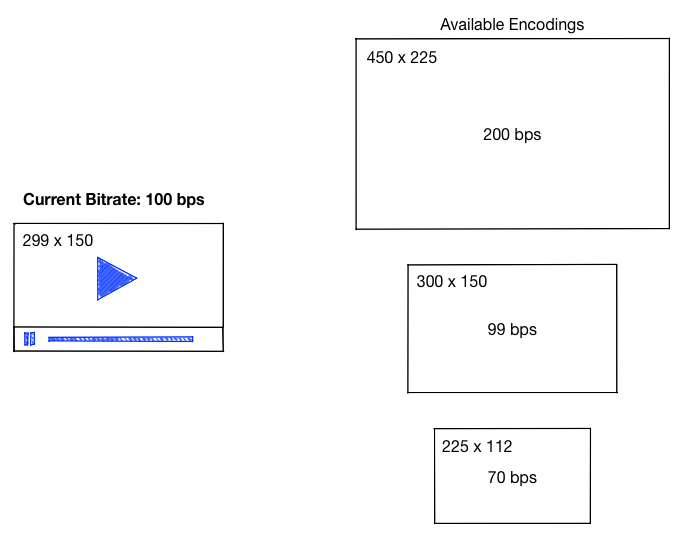
\includegraphics[width=1.0\linewidth]{images/chapter4/bitrate-switching-1.png}\hfill
 \caption[xxxxxxxxx]{xxxxxxxxxxxxx}
 \label{fig:fourV}
\end{figure}


First, we filter out all the renditions that have a higher bitrate than the new measurement:


\begin{figure}[htb] %  figure placement: here, top, bottom
 \centering
 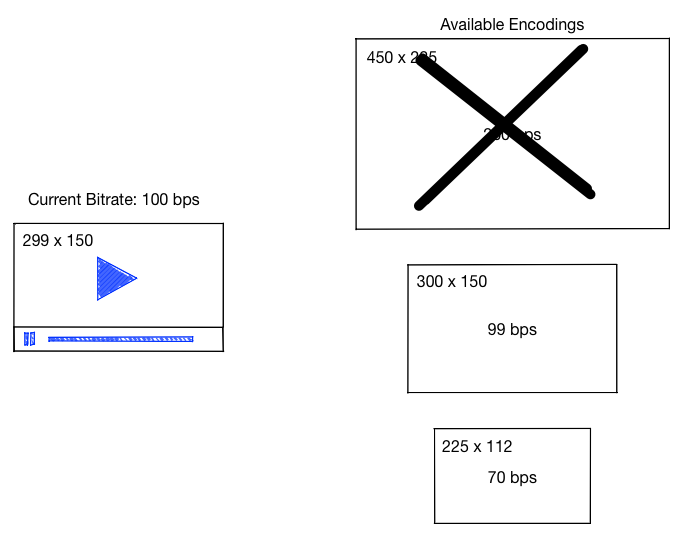
\includegraphics[width=1.0\linewidth]{images/chapter4/bitrate-switching-2.png}\hfill
 \caption[xxxxxxxxx]{xxxxxxxxxxxxx}
 \label{fig:fourV}
\end{figure}

Then we get rid of any renditions that are bigger than the current player dimensions:


\begin{figure}[htb] %  figure placement: here, top, bottom
 \centering
 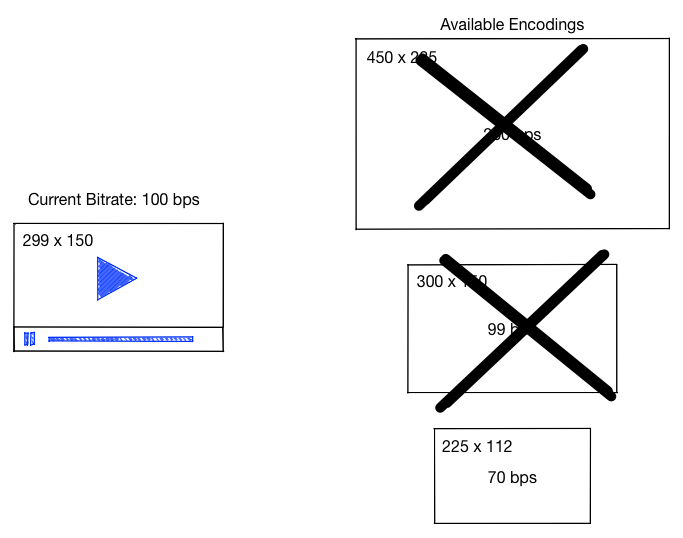
\includegraphics[width=1.0\linewidth]{images/chapter4/bitrate-switching-3.png}\hfill
 \caption[xxxxxxxxx]{xxxxxxxxxxxxx}
 \label{fig:fourV}
\end{figure}

We don't want to signficant quality drop just because your player is one pixel too small, so we add back in the next highest resolution. The highest bitrate rendition that remains is the one that gets used:


\begin{figure}[htb] %  figure placement: here, top, bottom
 \centering
 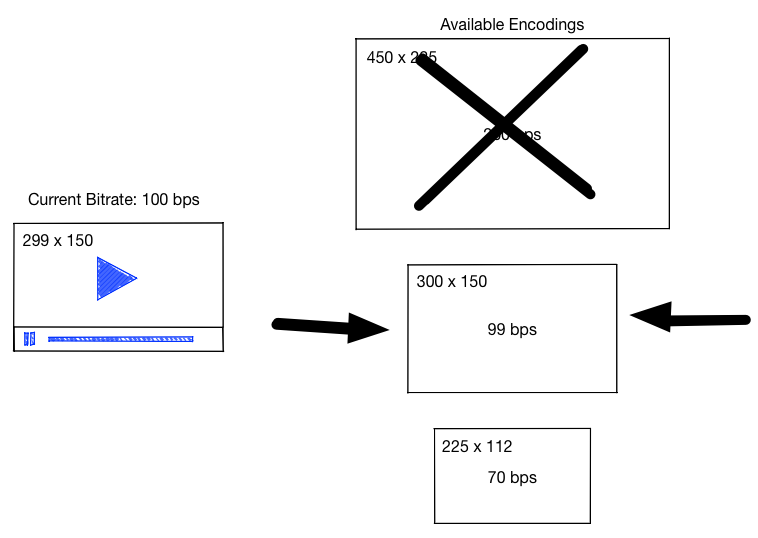
\includegraphics[width=1.0\linewidth]{images/chapter4/bitrate-switching-4.png}\hfill
 \caption[xxxxxxxxx]{xxxxxxxxxxxxx}
 \label{fig:fourV}
\end{figure}


If it turns out no rendition is acceptable based on the filtering described above, the first encoding listed in the master playlist will be used.


\newpage